\documentclass[letterpaper,10pt,titlepage,draftclsnofoot,onecolumn,onesided] {IEEEtran}
\usepackage{listings}
\usepackage{underscore}
\usepackage[bookmarks=true]{hyperref}
\usepackage[utf8]{inputenc}
\usepackage[english]{babel}
\usepackage{hyperref}
\usepackage{titling}
\usepackage{graphicx}
\usepackage[noadjust]{cite}
\nocite{*}
\graphicspath{ {images/} }

\hypersetup{
    bookmarks=false,    % show bookmarks bar?
    pdftitle={Software Requirement Specification},    % title
    pdfauthor={Cramer Smith, Sam Lichlyter, Eric Winkler, Zach Schneider},                     % author
    pdfsubject={Requirements Document},                        % subject of the document
    pdfkeywords={IFT, Requirements, Postal}, % list of keywords
    colorlinks=true,       % false: boxed links; true: colored links
    linkcolor=black,       % color of internal links
    citecolor=black,       % color of links to bibliography
    filecolor=black,        % color of file links
    urlcolor=blue,        % color of external links
    linktoc=page            % only page is linked
} 

\begin{document}

\markboth{Oregon State University}{Requirements Document for Postal}

\title{\Huge{\bfseries{\textsf{Requirements Document for Postal}}}}
\author{Cramer Smith, Sam Lichlyter, Eric Winkler, Zach Schneider}

\maketitle
\vfill
\begin{abstract}

Developer tools are often complex pieces of software. Gathering and manipulating useful information for a programmer can often be a slow and costly process. By implementing Information Foraging Theory design patterns in the creation of these tools, the information collected may be more useful or produced faster. Information Foraging Theory is the theory and math behind the choices people make to maximize the value of the information they find versus the cost of getting that information. Our aim is to develop a tool that will act as a proof of concept to this idea and increase developer efficiency. Implementing multiple IFT design patterns, we will create a developer tool that helps enforce and maintain code structure. 

\end{abstract}
\vfill

\pagebreak

\tableofcontents

\pagebreak

\section{Introduction}

The Postal extension is being made with two goals in mind. The first being to provide evidence that the use of IFT Design Patterns in the production of developer tools is beneficial. The second is to create a tool that will help developers write and maintain clean code bases for websites.
The Postal extension will do this by giving the user friendly reminders and suggestions of the best practices of the current language that they are using and by providing a visual representation of their project's code base.

\subsection{Purpose}
The purpose of the Software Requirements Specification of the Postal extension is describe the ways that functionality and way that the extension will be used by our target user. 
As well as being a guide line for us as developers steering us toward developing the correct functionality and making sure that we stick to a loose time line going through with the project.
The hope is that this document will help us and our steak holders have a better understand of what it is our project's purpose actually is.

\subsection{Scope}
The Postal Project is to developed by Research Experience Undergraduates under the lead of Christopher Scaffidi. 
The project will consist of a Visual studio code extension.
The purpose of this extension is to help new web developers develop good practices in their styling of code.
We hope to help new developers avoid the same mistakes we made when we first started web development with very confusing CSS pages and way too many confusing HTML pages and poorly defined JavaScript files.
The scope of our project is to create an extension to be used on Visual Studio Code. 
This extension will be able to look at the code that the user is editing and the program will be able to give them suggestions based on the the W3 standards. 

\subsection{Definitions, Acronyms, and Abbreviations}
\setlength\parindent{0pt}Information Foraging Theory (IFT): \\
An approach to the analysis of human activities involving information access technologies. The theory derives from optimal foraging theory in biology and anthropology, which analyzes the adaptive value of food-foraging strategies.\cite{xeroxift}\\\\
IFT Design Patterns: \\
General, reusable solutions to common design problems.\cite{iftwiki}\\\\
Visualize Topology: \\
To reveal the structure of the information topology to help developers more easily navigate structural relationships, backtrack, and make better decisions about which patches to visit.\cite{iftwiki}\\
Notifier: \\
Automatically notify the developer of a change in an information patch which may result in prey desired by the developer appearing in the patch.\cite{iftwiki}\\\\
Dashboard: \\
Generate an information patch in which a developer can become aware of links that lead to continually changing information patches relevant to his or her work.\cite{iftwiki}\\\\
Gather Together: \\
Enable a developer to assemble information features from disparate patches into a single patch, thus reducing the cost of navigation between those features.\cite{iftwiki}\\\\
Reduce Duplicate Information: \\
Enable developers to quickly forage by reducing the size of the topology. Here, the size of the topology is reduced by eliminating nodes with duplicate information.\cite{iftwiki}\\\\
VSC, VS Code:\\
Visual Studio Code.\\\\
IRB: \\
Institutional Review Board.\\\\
File Map: \\
The graphical user interface for visualizing project files and links, as well as errors inside code.

\subsection{References}
\bibliographystyle{IEEEtran}
\bibliography{requirements}

\subsection{Overview}
For the rest of this document we will be looking at detailed requirements for the Postal Project. 
This will be an overall description of what the product means to the people that the Postal extension means to the people that will be using the project and why they are using and how it will help them in their development processes. 
The next subsection will go over the specific requirements that steer the development process and keep the team focused on the goals specified in this document.   

\section{Overall Description}
Postal is an extension for Visual Studio code  that is supposed to help beginner developers while they make websites using HTML, CSS and JavaScript. 

\subsection{Product Perspective}
The product is aimed toward people that are learning web development we hope that as a user they find that our tool makes the development process more educational and easier for them to understand.

\subsubsection{System Interfaces}
Visual Studio Code was chosen as the sole system interface for Postal.
VSC is free, lightweight, and open source, making it accessible to both developers and users of this development tool.

\subsubsection{User Interfaces}
The main interface that we plan to implement is a graphical representation of the users files. 
We want the users to be able to quickly navigate through a visual representation of their files in hopes that this will give new developers a different way of thinking about their projects.
This different perspective will hopefully encourage the user to implement better file structure and organization in their projects.

\subsubsection{Software Interfaces}
From our end we would be interfacing with the VSC extension API. To create and develop our code and we will be using the npm tool that is included in Node.js and using a code generator called 'yoeman'. We will use yo to generate a skeleton of files which we will then be able to edit and make into an extension using JavaScript. The skeleton code will be the base of what we build the rest of the extension on. 

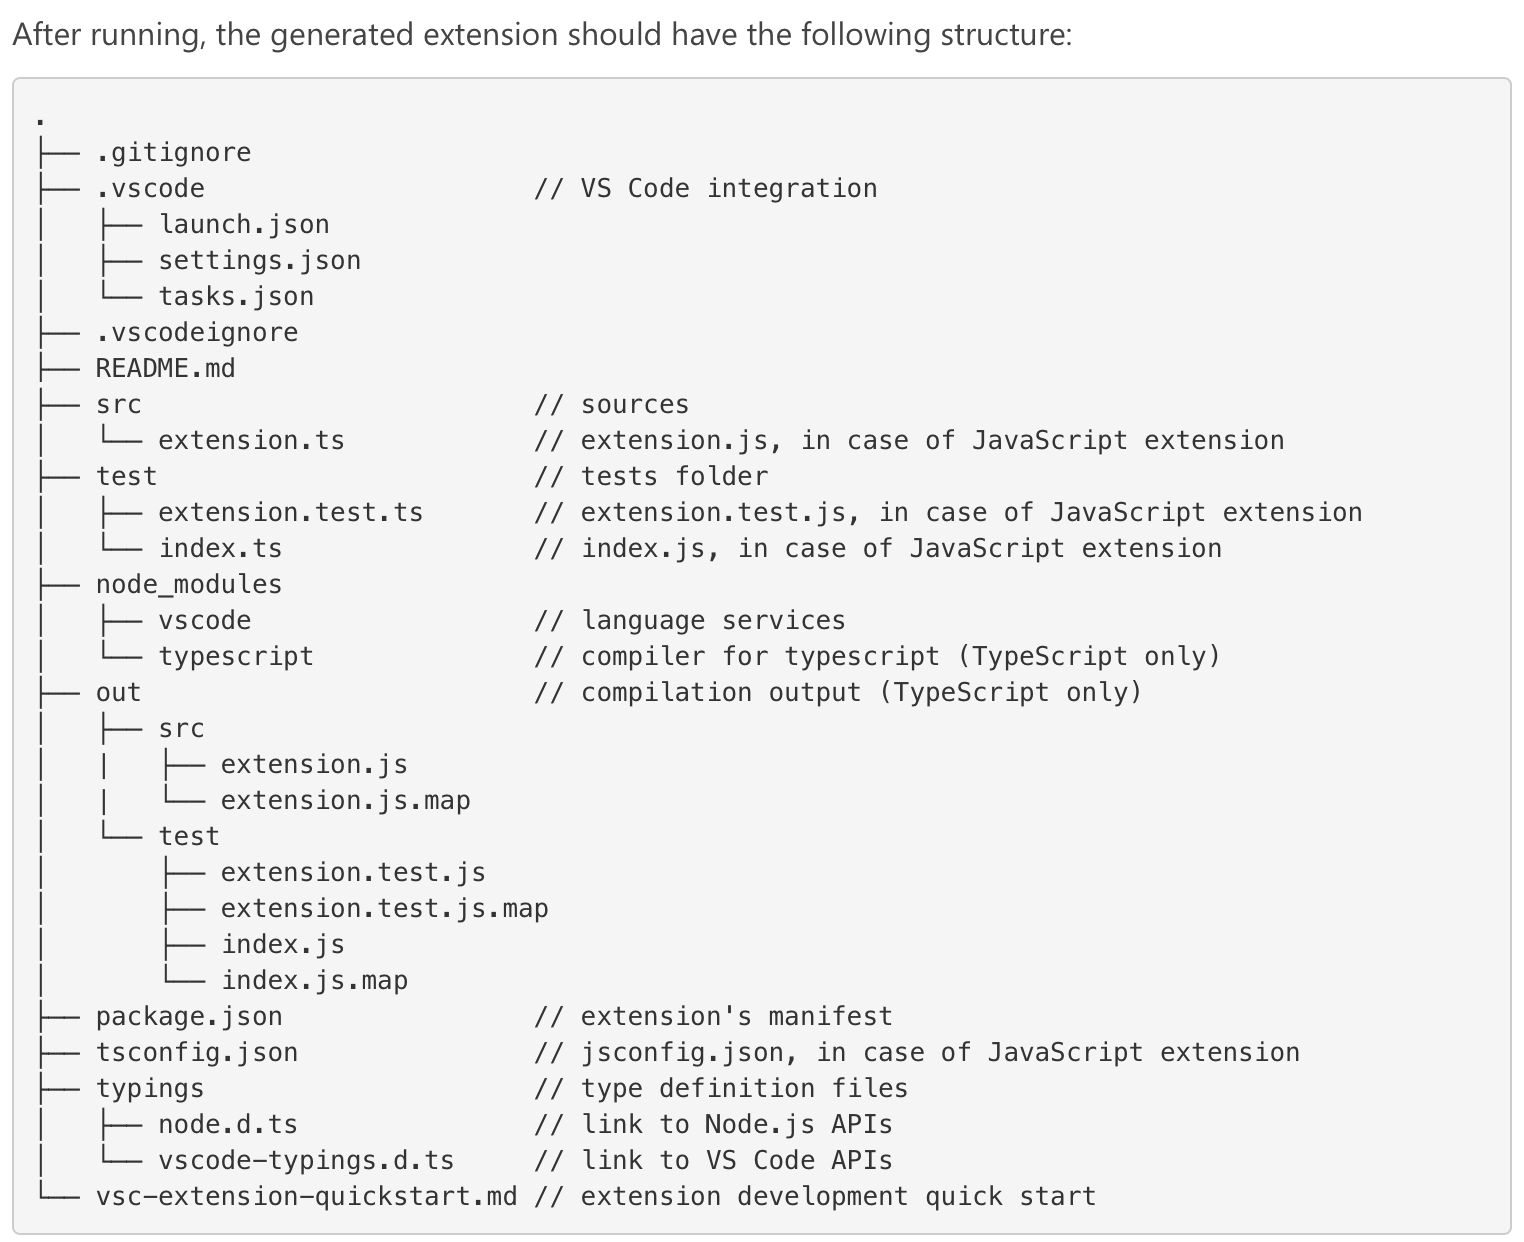
\includegraphics[scale=0.5]{fileStructure.png}
\subsubsection{Communication Interfaces}
The only communication interface that Postal will require is an ability to download the extension from the VS Code Extension Marketplace. 

\subsubsection{Operations}
TODO: Uncertain what specific operations the users will follow.

\subsection{Product Functions}
From a functional perspective, Postal will largely do two things: Provide the user with a visual perspective of their project folder and parse HTML, CSS and JavaScript files for bad coding practices and information to feed into the visual interface. 
The visual interface component will be a separate window referred to as the ?File Map?. This window will scan the directory of the currently open project and create a visual representation of the files in the folder. The representation will also feature indicators of errors that the parser detects in files and visually display any links between files.
The parser will read the HTML, CSS and JavaScript files in the user?s project folder and look for specific violations of rules the defined in the system. These rules will be based on W3?s best practices guidelines. Additionally, the parser will ignore any lines of code that marked in an exception list, allowing the user to break rules in the case that they have to.
Along with our product completing the aforementioned requirements, it also needs to be implemented using the IFT Design Patterns we also mentioned previously in this document.
The exention will be able to parse and interpret a code projects with up to one hundred thousand lines of code quickly without noticeable lag. 
More specifically the extension will be able to handle files of this size with less than one second of lag.
The entire extension should run seamlessly with the user taking little to no notice that our processes are running. 
The user should experience little to no lag while our extension is running depending on the power of their personal machine.
We will assume that an average user is using a computer with at least two gigabytes of ram. 
The project inherently won't have any safety requirements. 

\subsection{User Characteristics}
Users of Postal will be web developers and computer science students with some level of prior development experience, though prior knowledge will not be required. The users will be familiar with the concepts surrounding programming languages and markup languages, such as HTML, CSS and JavaScript. 
Users will be familiar with file systems, such that the visualization within Postal will enhance understanding of project structure. 
Users should have a basic understanding of debugging techniques that will be aided by the error recognition and highlighting within Postal.

\subsection{Constraints}
The Postal extension for VSC will be constrained chiefly by software and programming language level barriers.
As this extension will be primarily written in JavaScript (ECMAScript2016 standard, specifically), it will be bound by any functional or design limitations that exist within that programming language. 
Additionally, all Postal functionality must be possible within the VSC environment. 
VSC does not detail any notable constraints in its documentation that would conflict with the goals of Postal at this time. 
Finally, the file visualization and linking features of postal will be reliant on read, write and execute permissions within the scope of project loaded into VSC at that time. If any user's operating system restricts Postal access to any of those file system features, that operating system will also be a constraint to proper function.

\subsection{Assumptions and Dependencies}
The successful development of Postal assumes that Microsoft will not update Visual Studio Code in such a manner that breaks the function of the Postal extension. It is also assumed that VSC will continue to support the operating systems used in development, testing, and utilization of Postal.

\subsection{Apportionment of Requirements}
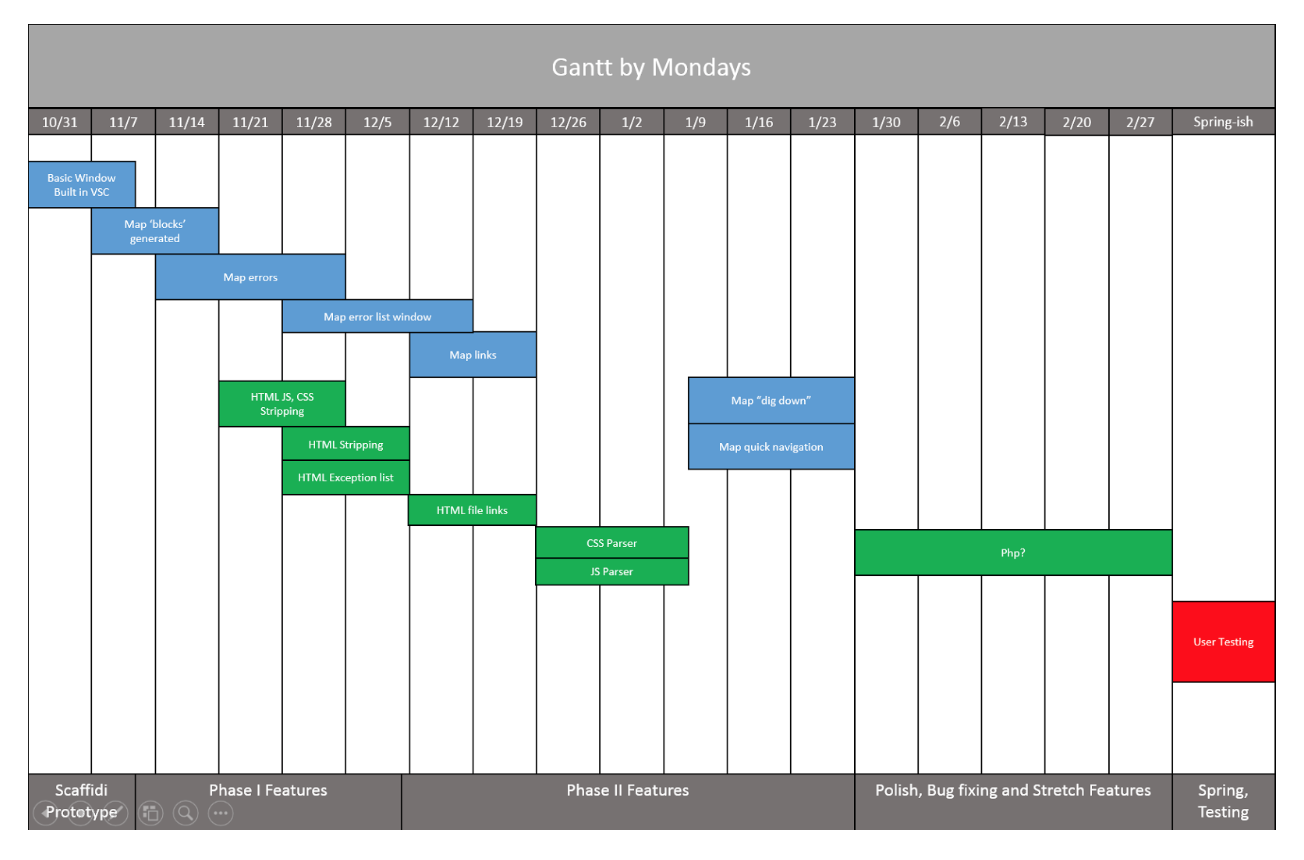
\includegraphics[scale=0.7]{gantt.png}

\section{Specific Requirements}

\subsection{External Interfaces}
The primary interface of the extension will be a window within the Visual Studio Code environment. This window will contain two main elements (the File Map and the Error List) as well as a toolbar for options.
\\
The File Map is a visualization of the user's project. When a project is opened within VSC, the extension will automatically populate the map by scanning the directory of the opened solution. This map will display each file found in the project directory in an organized fashion. The map will also feature options to display a visual indicator of links and calls between files in the directory (for example, if an HTML page has an image embedded in it, the link option would indicate a link between the HTML and image files) as well as an option to display an indicator of the location of errors within the GUI.
\\
The user will also be able to interact with the File Map by ``digging down'' into a file. This process will allow a user to click on a visualized file and have the map display more details about that file. For example, if an HTML file is clicked on within the map, the UI will update and visualize details of the file like divs and links as their own objects. If the above mentioned error option is enabled, the object containing the error would indicate that.
\\
The Error list is a list which displays all errors that the parser detected during its last run. The User will be able to click on a particular error in this list which will then trigger the extension to navigate the user to that particular error in the code. Additionally if the user hovers over a particular error, the corresponding location in the file map will be highlighted.

\subsection{Functions}

\subsubsection{Parser Related Functionality}
\begin{itemize}
	\item Functionality capable of parsing JavaScript, HTML and CSS documents. As parsing occurs, particular instances of code that break rules defined in the system will be flagged. Flagged lines will be visualized in the File Map.
	\item The system must have a method for storing rules that will be used by the parser to determine if a line of code should be marked as an error. Many of these rules will be based on W3 best practices for the particular parser.
	\item The system must have an editable list of exceptions. Exceptions are defined segments of code that may break a parsing rule, but because it was either intentional or necessary, should not throw an error.
	\item Current Parsing Rules for HTML:
		\begin{itemize}
			\item Flag JavaScript and CSS code that is not in the exception list.
			\item Make a note of each use of another file within the HTML file. This will be used to visualize links between files in the map.
		\end{itemize}
	\item Current Parsing Rules for CSS:
		\begin{itemize}
			\item Flag styles that can be optimized (ids vs. Classes).
			\item Flag redundant definitions.
			\item Do not flag code in the exception list.
		\end{itemize}
	\item Current Parsing Rules for JS:
		\begin{itemize}
			\item Flag Global variables that are not defined at the top of a file.
		\end{itemize}
\end{itemize}

\subsubsection{File Map Functionality}
\begin{itemize}
	\item Display in a visual, chart-like manner all files in the project directory.
    \item Display links and calls between files. This option can be turned off by the user.
    \item Display indicators of errors (broken rules) at the corresponding location within the map. This option can be turned off by the user.
    \item The system must allow for the Dig Down functionality. When an object in the map is clicked on, the map will update to display the object in more detail. Details will often be their own object. Error indicators will be updated.
    \item Display an error list adjacent to the file map. Errors will be organized by location.
    \begin{itemize}
    	\item If the user hovers over a particular error in the list, the corresponding location in the file map will be 	highlighted.
        \item If the user clicks on a particular error in the list, the extension will navigate the user to the location of the error in the code.
    \end{itemize}
\end{itemize}

\subsection{Performance Requirements}
Our product will be able to support as many projects as each user has. 
Given a web site project consisting of less than thirty HTML files, five CSS files, and ten JavaScript files, our product should complete its analysis in less than a second. 
This example should be a pretty standard setup for most intermediate web developers.
\\
Our parser should complete each HTML file in less than 1/5th of a second and each CSS and JavaScript file in less than 1/10th of a second.

\subsubsection{Standards Compliance}
Other than the standards set forth by the VSC extension API, there are no overarching standards our product needs to comply with.
The plan is to test our product with people following the IRB protocols, and the testing will follow their safety requirements regarding the testers information.

\subsection{Software System Attributes}
The software that we will use is Visual Studio Code. We are making an extension for this base

\subsubsection{Reliability}
Postal should complete its analysis for 95\% of the projects it is given. It should also satisfy the performance requirements 95\% of the time.   


\section{Other Requirements}

\subsection{Appendix A: Glossary}
%see https://en.wikibooks.org/wiki/LaTeX/Glossary

\subsection{Appendix B: Analysis Models}

\subsection{Appendix C: To Be Determined List}

\end{document}
